
Una empresa de turismo que vende excursiones desea realizar una campaña publicitaria en diferentes vuelos comerciales con el objetivo de llegar a todos los viajeros que parten del país A y que se dirigen al país B. Estos viajeros utilizan diferentes rutas (algunos vuelos directos, otros armando sus propios recorridos intermedios). Se conoce para una semana determinada todos los vuelos entre los diferentes aeropuertos con sus diferentes capacidades. Además parten del supuesto que durante ese periodo la afluencia entre A y B no se verá disminuida por viajes entre otros destinos.

Desean determinar en qué trayectos simples (trayecto de un viaje que inicia desde un aeropuerto y termina en otro) poner publicidad de forma de alcanzar a TODAS las personas que tienen el destino inicial A y el destino final B. Pero además desean que siempre que sea posible seleccionen la combinación que tenga el menor número de vuelos comerciales. Esto es porque pagan tanto por cantidad de vuelos como por pasajeros que cumplan con la condición de ser del país de origen A y con destino final B. \\

Se pide:

1. Proponer una solución algorítmica que resuelva el problema de forma eficiente. Explicarla paso a paso. Utilice diagramas para representarla.

2. Plantear la solución como si fuese una reducción de problema. ¿Puede afirmar que corresponde a una reducción polinomial? Justificar.

3. ¿Podría asegurar que su solución es óptima?

4. Programe la solución

5. Compare la complejidad temporal y espacial de su solución programada con la teórica. ¿Es la misma o difiere? \\

\section{Solución algorítimica que resuelve el problema de forma eficiente. Paso a paso} Modelamos el problema con un grafo donde los vuelos son aristas cuyos pesos son sus capacidades máximas y los aeropuertos son vértices. Luego, resolvemos mediante el algoritmo de Edmonds-Karps de la siguiente manera: \\

 \begin{center}
    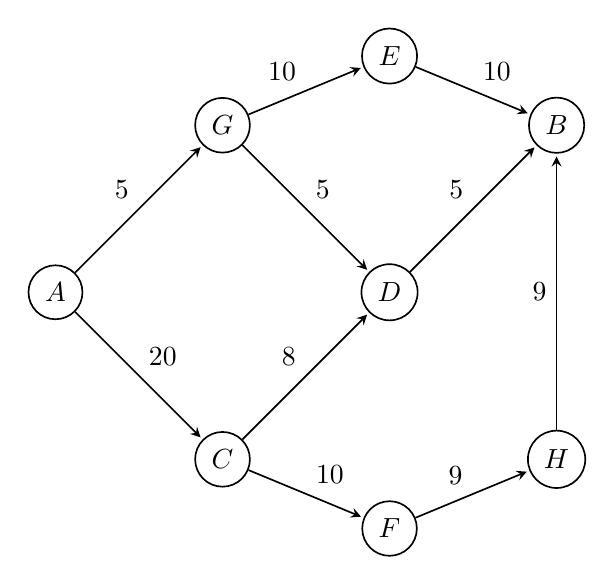
\begin{tikzpicture}[
            thick, 
            main/.style = {draw, circle}, 
            > = stealth, % arrow head style
            shorten > = 1pt, % don't touch arrow head to node
            auto,
            node distance = 3cm, % distance between nodes
            semithick % line style
        ]
        \node[main] (a) {$A$};
        \node[main] (g) [above right of=a] {$G$};
        \node[main] (c) [below right of=a] {$C$}; 
        \node[main] (d) [below right of=g] {$D$};
        \node[main] (e) [above of=d] {$E$};
        \node[main] (f) [below of=d] {$F$};
        \node[main] (b) [above right of=d] {$B$};
        \node[main] (h) [below right of=d] {$H$};

        \path[->] (a) edge node {5} (g);
        \path[->] (a) edge node {20} (c);
        \path[->] (c) edge node {10} (f);
        \path[->] (c) edge node {8} (d);
        \path[->] (g) edge node {5} (d);
        \path[->] (g) edge node {10} (e);
        \path[->] (e) edge node {10} (b);
        \path[->] (d) edge node {5} (b);
        \path[->] (f) edge node {9} (h);
        \path[->] (h) edge node {9} (b);
    \end{tikzpicture} 
\end{center}

\begin{enumerate}
\item Se utiliza el algoritmo de BFS (Breadth First Search o Búsqueda en Anchura) para encontrar el camino mínimo de A a B, solo considerando las aristas que no estén saturadas. \\

 \begin{center}
    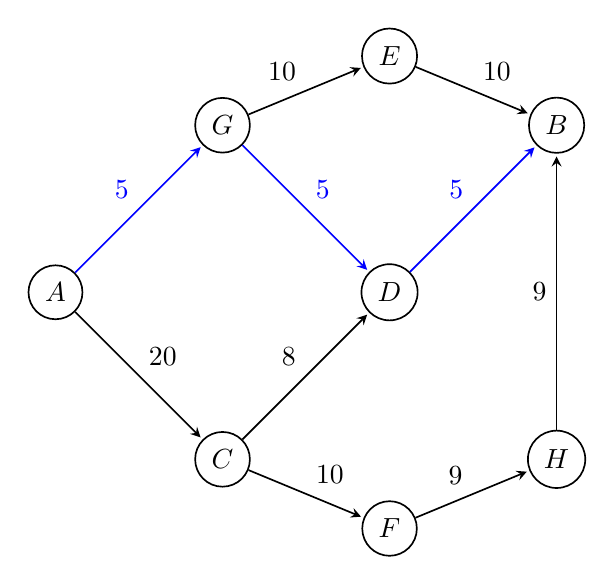
\begin{tikzpicture}[
            thick, 
            main/.style = {draw, circle}, 
            > = stealth, % arrow head style
            shorten > = 1pt, % don't touch arrow head to node
            auto,
            node distance = 3cm, % distance between nodes
            semithick % line style
        ]
        \node[main] (a) {$A$};
        \node[main] (g) [above right of=a] {$G$};
        \node[main] (c) [below right of=a] {$C$}; 
        \node[main] (d) [below right of=g] {$D$};
        \node[main] (e) [above of=d] {$E$};
        \node[main] (f) [below of=d] {$F$};
        \node[main] (b) [above right of=d] {$B$};
        \node[main] (h) [below right of=d] {$H$};

        \path[blue,->] (a) edge node {5} (g);
        \path[->] (a) edge node {20} (c);
        \path[->] (c) edge node {10} (f);
        \path[->] (c) edge node {8} (d);
        \path[->, blue] (g) edge node {5} (d);
        \path[->] (g) edge node {10} (e);
        \path[->] (e) edge node {10} (b);
        \path[->, blue] (d) edge node {5} (b);
        \path[->] (f) edge node {9} (h);
        \path[->] (h) edge node {9} (b);
    \end{tikzpicture} 
\end{center}

\item Se calcula la menor capacidad en el camino, a la cual llamamos cuello de botella, que le resta a la capacidad de la arista original y se le suma a la capacidad de la arista residual (la arista en el sentido contrario, de capacidad máxima 0). \\

 \begin{center}
    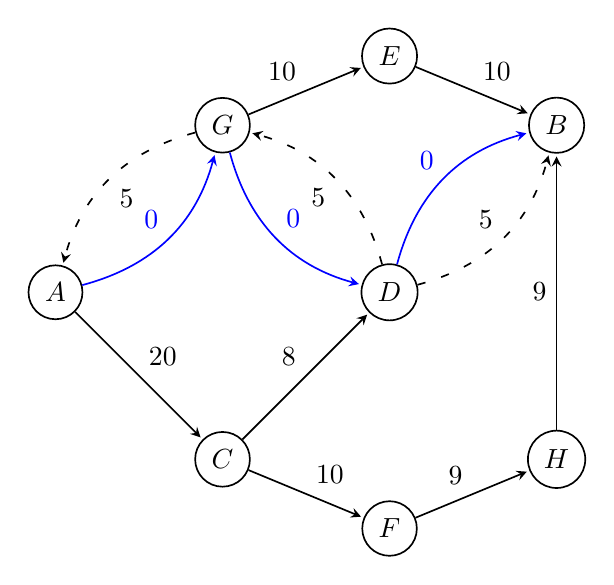
\begin{tikzpicture}[
            thick, 
            main/.style = {draw, circle}, 
            > = stealth, % arrow head style
            shorten > = 1pt, % don't touch arrow head to node
            auto,
            node distance = 3cm, % distance between nodes
            semithick % line style
        ]
        \node[main] (a) {$A$};
        \node[main] (g) [above right of=a] {$G$};
        \node[main] (c) [below right of=a] {$C$}; 
        \node[main] (d) [below right of=g] {$D$};
        \node[main] (e) [above of=d] {$E$};
        \node[main] (f) [below of=d] {$F$};
        \node[main] (b) [above right of=d] {$B$};
        \node[main] (h) [below right of=d] {$H$};

        \path[blue,->] (a) edge[bend right] node {0} (g);
        \path[->] (a) edge node {20} (c);
        \path[->] (c) edge node {10} (f);
        \path[->] (c) edge node {8} (d);
        \path[->, blue] (g) edge[bend right] node {0} (d);
        \path[->] (g) edge node {10} (e);
        \path[->] (e) edge node {10} (b);
        \path[->, blue] (d) edge[bend left] node {0} (b);
        \path[->] (f) edge node {9} (h);
        \path[->] (h) edge node {9} (b);
        
        \path[->, loosely dashed] (g) edge[bend right] node {5} (a);
        \path[->, loosely dashed] (d) edge[bend right] node {5} (g);
        \path[->, loosely dashed] (d) edge[bend right] node {5} (b);
    \end{tikzpicture} 
\end{center}

\item Se repiten los pasos 1-2 hasta que no queden caminos de A a B con capacidad disponible. \\

 \begin{center}
    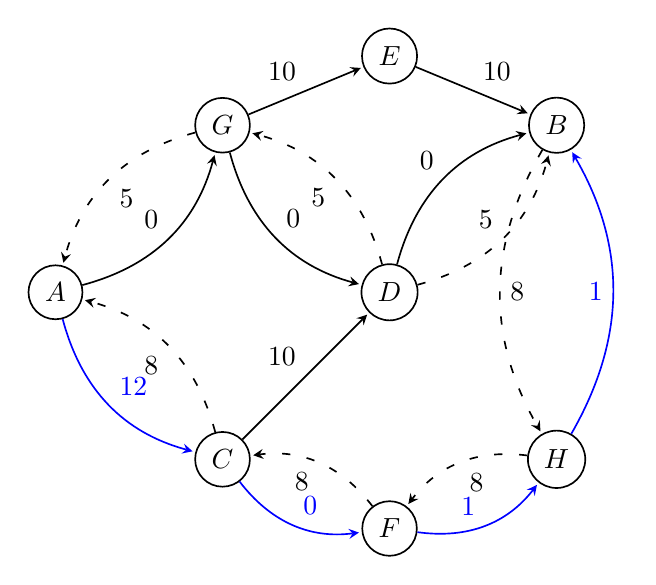
\begin{tikzpicture}[
            thick, 
            main/.style = {draw, circle}, 
            > = stealth, % arrow head style
            shorten > = 1pt, % don't touch arrow head to node
            auto,
            node distance = 3cm, % distance between nodes
            semithick % line style
        ]
        \node[main] (a) {$A$};
        \node[main] (g) [above right of=a] {$G$};
        \node[main] (c) [below right of=a] {$C$}; 
        \node[main] (d) [below right of=g] {$D$};
        \node[main] (e) [above of=d] {$E$};
        \node[main] (f) [below of=d] {$F$};
        \node[main] (b) [above right of=d] {$B$};
        \node[main] (h) [below right of=d] {$H$};

        \path[->] (a) edge[bend right] node {0} (g);
        \path[->, blue] (a) edge[bend right] node {12} (c);
        \path[->, blue] (c) edge[bend right] node {0} (f);
        \path[->] (c) edge node {10} (d);
        \path[->] (g) edge[bend right] node {0} (d);
        \path[->] (g) edge node {10} (e);
        \path[->] (e) edge node {10} (b);
        \path[->] (d) edge[bend left] node {0} (b);
        \path[->, blue] (f) edge[bend right] node {1} (h);
        \path[->, blue] (h) edge[bend right] node {1} (b);
        
        \path[->, loosely dashed] (g) edge[bend right] node {5} (a);
        \path[->, loosely dashed] (d) edge[bend right] node {5} (g);
        \path[->, loosely dashed] (d) edge[bend right] node {5} (b);
        
        \path[->, loosely dashed] (c) edge[bend right] node {8} (a);
        \path[->, loosely dashed] (f) edge[bend right] node {8} (c);
        \path[->, loosely dashed] (h) edge[bend right] node {8} (f);
        \path[->, loosely dashed] (b) edge[bend right] node {8} (h);
    \end{tikzpicture} 
\end{center}
 \begin{center}
    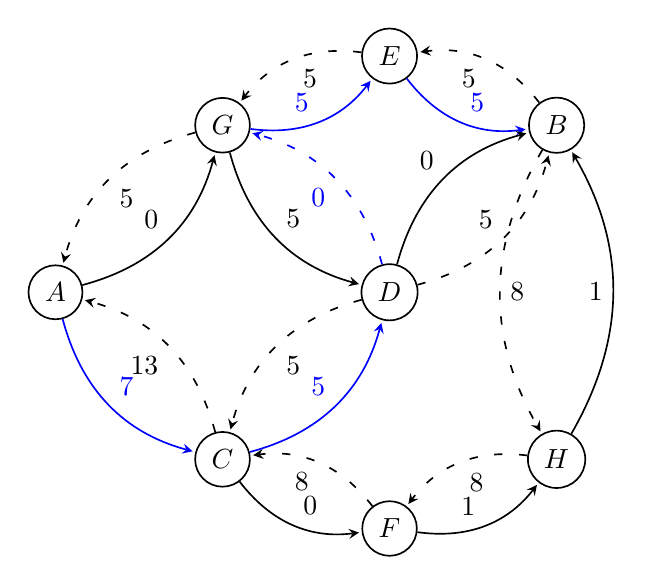
\begin{tikzpicture}[
            thick, 
            main/.style = {draw, circle}, 
            > = stealth, % arrow head style
            shorten > = 1pt, % don't touch arrow head to node
            auto,
            node distance = 3cm, % distance between nodes
            semithick % line style
        ]
        \node[main] (a) {$A$};
        \node[main] (g) [above right of=a] {$G$};
        \node[main] (c) [below right of=a] {$C$}; 
        \node[main] (d) [below right of=g] {$D$};
        \node[main] (e) [above of=d] {$E$};
        \node[main] (f) [below of=d] {$F$};
        \node[main] (b) [above right of=d] {$B$};
        \node[main] (h) [below right of=d] {$H$};

        \path[->] (a) edge[bend right] node {0} (g);
        \path[->, blue] (a) edge[bend right] node {7} (c);
        \path[->] (c) edge[bend right] node {0} (f);
        \path[->, blue] (c) edge[bend right] node {5} (d);
        \path[->] (g) edge[bend right] node {5} (d);
        \path[->, blue] (g) edge[bend right] node {5} (e);
        \path[->, blue] (e) edge[bend right] node {5} (b);
        \path[->] (d) edge[bend left] node {0} (b);
        \path[->] (f) edge[bend right] node {1} (h);
        \path[->] (h) edge[bend right] node {1} (b);
        
        \path[->, loosely dashed] (g) edge[bend right] node {5} (a);
        \path[->, loosely dashed, blue] (d) edge[bend right] node {0} (g);
        \path[->, loosely dashed] (d) edge[bend right] node {5} (b);
        
        \path[->, loosely dashed] (c) edge[bend right] node {13} (a);
        \path[->, loosely dashed] (f) edge[bend right] node {8} (c);
        \path[->, loosely dashed] (h) edge[bend right] node {8} (f);
        \path[->, loosely dashed] (b) edge[bend right] node {8} (h);
        
        \path[->, loosely dashed] (d) edge[bend right] node {5} (c);
        \path[->, loosely dashed] (b) edge[bend right] node {5} (e);
        \path[->, loosely dashed] (e) edge[bend right] node {5} (g);
    \end{tikzpicture} 
\end{center}
Finalmente, tenemos el grafo residual y el flujo máximo que es la suma de todos los cuellos de botella. \\
\item Utilizando el grafo residual obtenemos el corte mínimo de la siguiente manera: \\
    \begin{enumerate}
    \item Dividimos el grafo en 2 grupos, el grupo A será el que contenga todos los vértices accesibles desde el vértice fuente. El grupo B tendrá al resto de vértices. \\
    \item Observando el grafo original, diremos que todas las aristas que conecten un vértice del grupo A con un vértice del grupo B, están en el corte mínimo. \\
    \end{enumerate}

\item Finalmente, las publicidades serán colocadas en todas las aristas que estén en el corte mínimo.
\end{enumerate}

\section{Solución algorítima como si fuese una reducción del problema} Acá va el 1.2
\section{Optimalidad de la solución}
La solución propuesta por Edmonds-Karp es óptima ya que el algoritmo termina cuando no quedan caminos de A a B sin saturar, el flujo calculado es el máximo. 

\section{\href{https://github.com/ilitteri/7529-TDA-1/blob/master/tp3/README.md}{Solución Programada (clickeame)}}

\section{Comparación temporal y espacial de la solución programada}
La complejidad teórica del algoritmo de Edmons-Karp es $O(VE^2)$ ya que utiliza BFS para encontrar los caminos. La complejidad temporal del corte mínimo es $O(V^2)$ ya que en el peor de los casos todos los vértices están conectados ente sí y las aristas que conectan con el destino son las que generan el cuello de botella. La complejidad total de ambas operaciones es $O(VE^2)$. \\

Con respecto a su complejidad espacial, se utiliza un grafo residual de V.2E y BFS utiliza una cola de a lo sumo V elementos, por lo que la complejidad espacial de Edmons-Karp es $O(VE)$. La complejidad espacial del corte mínimo es $O(V)$ ya que en el peor de los casos hay V vértices en el grupo A. Por lo tanto, la complejidad temporal total de la operación es $O(VE)$ \\

Las complejidades temporal y espacial de la solución programada coinciden con las teóricas.